\chapter{Introduction}
\graphicspath{{introduction/figures/}{introduction/}}


\section{The Standard Model of Particle Physics}

The Standard Model of particles and fields (SM) describes the most basic constituents of matter and their dynamics, as currently known. 
It is built upon the hypothesis that fundamental, point-like particles exist (fermions) and that their interactions, via bosonic fields, can be described in a relativistic quantum field theoretical framework. 
Fundamental interactions are described in the SM by the gauge invariance principle, meaning that interactions will appear in the framework as gauge fields after imposing local and continuous (gauge) symmetries. 
An early example of this principle is the emergence of electromagnetism on the Schr�dinger equation by imposing a local and continuous $U(1)$ symmetry.

As of today, the SM described three types of interactions: 

\begin{description}
\item[The Strong Interaction] Also known as quantum chromodynamics or QCD. It appears in the SM via an $SU(3)$ gauge symmetry. This gauge group implies the existence of 8 gauge bosons, called gluons. Fermions particles that interact via QCD are called \textbf{quarks}, and are organized in triplets of a "color" charge. Fermions that do not interact via QCD are called \textbf{leptons}. 

\item[The Electromagnetic Interaction] It appears in the SM via an $U(1)$ gauge symmetry, with one gauge boson associated to it (photon). The particles that interact via the electromagnetic interaction have electric charge. 

\item[The Weak Interaction] Appears in the SM via an $SU(2)$ gauge symmetry. It has three different gauge bosons associated to it, two have electric charge: $W^{+}$ and $W^{-}$, while one is neutral: $Z^{0}$. The weak interaction charge is commonly called weak hypercharge.
\end{description}

The two last interactions have been further combined in a single theoretical model, called the electroweak interaction  \cite{weinberg_ew, salam_ew, glashow_ew}. 
It is based on the fact that, before a spontaneous symmetry breaking occurs, both interactions can be described by a single gauge group, namely $SU(2)\otimes U(1)$. 
A main ingredient of this unification process is the spontaneous symmetry breaking mechanism based on the Higgs field \cite{englert_brout,guralnik,higgs}. 

The organization of the field content of the SM was completed with the observation that both quarks and leptons are organized into three generations. 
The first generation of leptons contains the electron ($e$) and the electron neutrino ($\nu_e$), while the first generation of quarks contains the up quark ($u$) and the down quark ($d$). 
The second generation of leptons contains the muon ($\mu$) and the mu neutrino ($\nu_{\mu}$), while the second generation of quarks contains the charm quark ($c$) and the strange quark ($s$). 
The third generation of leptons contains the tau ($\tau$) and the tau neutrino ($\nu_{\tau}$), while the third generation of quarks contains the top quark ($t$) and the bottom quark ($b$). 
The generation structure is particularly important by noting that particles of the same family, with left-handed chirality, form a weak isospin doublet, while the right-handed fermions are weak singlets: 

\begin{equation}
\begin{array}{ccc}
L_{l}=\left(\begin{array}{c}
\nu_{e}\\
e
\end{array}\right)_{L}, & \left(\begin{array}{c}
\nu_{\mu}\\
\mu
\end{array}\right)_{L}, & \left(\begin{array}{c}
\nu_{\tau}\\
\tau
\end{array}\right)_{L};\\
\\
L_{q}=\left(\begin{array}{c}
u\\
d
\end{array}\right)_{L}, & \left(\begin{array}{c}
c\\
s
\end{array}\right)_{L}, & \left(\begin{array}{c}
t\\
b
\end{array}\right)_{L};
\end{array}
\end{equation}



\begin{equation}
R_l = e_{R},\,\mu_{R},\,\tau_{R};\, \, R_q = u_{R},\, d_{R},\, c_{R},\, s_{R},\, t_{R},\, b_{R}.
\end{equation}



\section{The Electroweak Theory of Glashow-Weinberg-Salam}

Through observations that date back to the early XX century, the electroweak interactions were built upon a set of experimental fundaments:

\begin{description}
\item[Universality] The weak interactions are blind with respect to quarks and leptons generations. This means that the coupling strength is the same to any of the three families described previously.
\item[Massless and Left-Handed Neutrinos] For the energy regime to which the SM addresses, the neutrinos are idealized as massless (even though experiments have proved that they do have mass, even if below eV scale), and they only exist (or only interact with the SM) in their left-handed chirality.
\item[Chirality] The electroweak interactions are not chiral, i.e., the structure of the theory should treat right-handed and left-handed particles differently.
\item[Mixing] The electroweak eigenstates of quarks is not the same as their mass eigenstates. Therefore, the electroweak interaction acts on mixed states of quarks mass eigenstates. This quark mixing is described by the CKM matrix.
\end{description}

The unified electroweak theory is based on the $SU(2)_{L}\otimes U(1)_{Y}$ gauge group. 
The indices $L$ and $Y$ address the fact that the $SU(2)$ gauge bosons ($\vec{B}_{\mu}$) will only act upon left-handed particles, while the $U(1)$ gauge boson ($A_{\mu}$) will couple to particles that contain weak hypercharge. 
After the spontaneous symmetry breaking, these four gauge bosons will become the three weak bosons and the photon. 
We can write a lagrangean, symmetric under this gauge group, as:

\begin{eqnarray} 
\label{eq_lag_lep_quark}
\mathcal{L}_{GWS} & = & \mathcal{L}_{Fermions}+\mathcal{L}_{Gauge}\nonumber \\
 & = & \left\{ \bar{R}i\gamma^{\mu}\left(\partial_{\mu}+i\frac{a}{2}A_{\mu}Y\right)R+\bar{L}i\gamma^{\mu}\left(\partial_{\mu}+i\frac{a}{2}A_{\mu}Y+i\frac{b}{2}\vec{\sigma}\cdot\vec{B}_{\mu}\right)L\right\} \label{eq:lag_YM}\\
 &  & -\frac{1}{4}\left\{ F_{\mu\nu}^{M}F_{M}^{\mu\nu}+f_{\mu\nu}f^{\mu\nu}\right\}, \nonumber 
\end{eqnarray}

where $R$ and $L$ represents the right-handed and left-handed fermions, respectively; $a$ and $b$ represents the coupling constants of the model; $\gamma$ and $\sigma$ represent the Dirac and Pauli matrices, respectively; and $F$ and $f$ are the field strengths tensors of the electroweak bosons.

\subsection{Spontaneous Symmetry Breaking and Mass Generation}

One important detail of the lagrangean in Equation \ref{eq_lag_lep_quark} is the fact that mass terms to the electroweak bosons are forbidden by gauge invariance. 
Particularly, classical mass terms such as $m_{B}^{2}\vec{B}_{\mu}\cdot\vec{B}^{\mu}$ violate the model's gauge symmetry given that $\vec{B}_{\mu}$ transforms as:

\begin{eqnarray}
B_{\mu}^{M} & \rightarrow & B_{\mu}^{M}+\frac{1}{b}\partial_{\mu}\alpha^{M}\left(x\right)+\epsilon_{\,\,\, NO}^{M}B_{\mu}^{N}B_{\mu}^{O}.\label{eq:transf_calibre}
\end{eqnarray}

The Higgs mechanism is the way the SM generates these mass terms while keeping the gauge invariance intact. 
In its non-Abelian form, it adds an $SU(2)_{L}$ scalar doublet field $\Phi$ and a quartic potential $V(\Phi)$ to the SM lagrangean described previously:

\begin{eqnarray}
\Phi & = & \left(\begin{array}{c}
\phi^{+}\\
\phi^{0}
\end{array}\right),\label{eq:campo_higgs}\\
V\left(\Phi\right) & = & \mu^{2}\Phi^{\dagger}\Phi+\lambda\left(\Phi^{\dagger}\Phi\right)^{2},\label{eq:higgs_pot}
\end{eqnarray}
with $\phi^{+}$ e $\phi^{0}$ as complex scalar fields.

As a doublet, the covariant derivative that acts upon $\Phi$ is similar to the one that acts on left-handed leptons:

\begin{equation}
D_\mu =\partial_{\mu}+i\frac{a}{2}A_{\mu}Y+i\frac{b}{2}\vec{\sigma}\cdot\vec{B}_{\mu}.
\end{equation}
Therefore, we can write the final SM lagrangean, including the Higgs mechanism, as:
\begin{equation}
\mathcal{L}_{Higgs+GSW}=\left(D\Phi\right)^{\dagger}\left(D\Phi\right)
+\mu^{2}\Phi^{\dagger}\Phi+\lambda\left(\Phi^{\dagger}\Phi\right)^{2}
+ \mathcal{L}_{GSW}. \label{eq:b_hi}
\end{equation}

The shape of $V\left(\Phi\right)$ depends on the values of $\mu$ and $\lambda$. 
Therefore, we can place bounds on these parameters based on the role $V\left(\Phi\right)$ must perform. 
First, $V\left(\Phi\right)$ must not have a global minimum at $|\Phi| \rightarrow \infty$, which means $\lambda > 0$. 
Second, in order to properly generate the gauge boson masses, the $V\left(\Phi\right)$ minimum must not be at zero. 
This is accomplished by setting $\mu^{2} < 0$, which creates a $V\left(\Phi\right)$ minimum at $|\Phi|=\sqrt{-\frac{\mu^2}{\lambda}}\equiv v$, also known as the electroweak vacuum expectation value. 
The found vacuum is spherically symmetric, meaning it remains unchanged by rotations such as $\Phi_{min}\rightarrow\exp\left(i\frac{\vec{\sigma}}{2}\cdot\vec{\xi}\right)\Phi_{min}$. 
With this fact, we can expand the Higgs field around its vacuum as:

\begin{eqnarray}
\Phi & \rightarrow & \frac{1}{\sqrt{2}}\left(\begin{array}{c}
0\\
v+H\left(x\right)
\end{array}\right),\label{eq:campo_higgs-1}
\end{eqnarray}
 
Writing this expression explicitly in the covariant derivative definition, calculating $\left(D\Phi\right)^{\dagger}\left(D\Phi\right)$ and gathering the terms involving the Higgs vacuum perturbation, we have:

\begin{equation} \label{higgs_int_old}
\left[\frac{1}{4}\left(aA_{\mu}-bB_{\mu}^{3}\right)^{2}+\frac{b^2}{4}\left(B_{\mu}^{1}-iB_{\mu}^{2}\right)\left(B_{\mu}^{1}+iB_{\mu}^{2}\right)\right]\left(\frac{1}{\sqrt{2}}\left(v+H\left(x\right)\right)\right)^{2}
\end{equation}

We can simplify this equation with the following redefinitions:

\begin{eqnarray}
W_{\mu}^{\pm} & = & \frac{1}{\sqrt{2}}\left(B_{\mu}^{1}\pm iB_{\mu}^{2}\right),\label{eq:cp1}\\
Z_{\mu}^{0} & = & \frac{bB_{\mu}^{3}-aA_{\mu}}{\sqrt{b^2+a^2}},\\
\mathcal{A_{\mu}} & = & \frac{bB_{\mu}^{3}+aA_{\mu}}{\sqrt{b^2+a^2}}.\label{eq:cp2}
\end{eqnarray}

Using these new field definitions, we can expand $\left(v+H\left(x\right)\right)^2$ in equation \ref{higgs_int_old} to obtain their couplings to the Higgs vacuum and the Higgs perturbation:

\begin{eqnarray} \label{zw_h_int}
\frac{v^2}{8}\left(b^2+a^2\right)Z_{\mu}^{0}Z^{0\mu}+\frac{v^2b^2}{8}W_{\mu}^{+}W^{-\mu} +\\
\frac{v}{8}\left(b^2+a^2\right)Z_{\mu}^{0}Z^{0\mu}H\left(x\right)+\frac{vb^2}{8}W_{\mu}^{+}W^{-\mu}H\left(x\right) \nonumber +\\
\frac{1}{8}\left(b^2+a^2\right)Z_{\mu}^{0}Z^{0\mu}H\left(x\right)H\left(x\right)+\frac{b^2}{8}W_{\mu}^{+}W^{-\mu}H\left(x\right)H\left(x\right). \nonumber
\end{eqnarray}

The first two terms in the equation above are canonical mass terms to the $Z^0$ and $W^\pm$ fields, but the field $\mathcal{A}$ remains massless. 
This takes the model back exactly to standard views on the weak interactions, with one massive neutral boson and two massive charged bosons, and on the electromagnetic interaction, with one massless neutral boson. 
The mass of the $Z^0$ and $W^\pm$ bosons can then be expressed based on the electroweak vacuum expectation value and on the electroweak couplings, the latter being well known experimentally, as: $m_{W}^{2}=\frac{v^{2}b^{2}}{4}$ and $m_{Z}^{2}=\frac{v^2}{4}\left(b^2+a^2\right)$. 
We can express $v^{2}$ as a function of $m_{W}$ and related it to the Fermi coupling constant ($G_F$), such that $v=\sqrt{\frac{-\mu^2}{\lambda}}=\left(\sqrt{2}G_{F}\right)^{1/2}\approx246\unit{GeV}$
\cite{pdg}, where $G_{F}$ is precisely obtained through muon lifetime measurements.

We can also investigate the shape of the Higgs potential after the vacuum has been fixed. 
Using the previous definition of $v$, we have:

\begin{eqnarray}
V\left(\Phi\right) & = & \frac{-v\lambda}{2}\left(v+H\left(x\right)\right)^{2}+\frac{\lambda}{4}\left(v+H\left(x\right)\right)^{4}\\
 & = & -\frac{\lambda v^{4}}{2}+\lambda v^{2}H^{2}\left(x\right)+\lambda vH^{3}\left(x\right)+\frac{\lambda}{4}H^{4}\left(x\right).\label{eq:higgs_pot_aberto}
\end{eqnarray}

The first important term in the equation above, $\lambda v^{2}H^{2}\left(x\right)$, can be interpreted as a mass term for a scalar field. 
This means that perturbations on the Higgs field around the vacuum will be realized as a scalar boson, the Higgs boson, with mass equal to  $m_{H}^{2}=2\lambda v^{2}$.
The following terms describe how the Higgs boson interacts with itself via triple and quartic couplings. 
It is interesting to note that the Higgs boson can be understood as an excitation on a transversal section of the original potential. 
The other degrees of freedom present in the theory, namely the longitudinal excitations along the direction in which the vacuum is symmetric, were "eaten" by the massless fields  $\vec{B}$ e $A$, as new degrees of freedom related to their masses.

%%%%%%%%%%%%%%%%%%%%%%%%%%%%%%%%%%%%%%%%%%%%%%%%%%%%%%%%%%%%%%%%%%%%%%%%%%%
%%%%%%%%%%%%%%%%%%%%%%%%%%%%%%%%%%%%%%%%%%%%%%%%%%%%%%%%%%%%%%%%%%%%%%%%%%%
%%%%%%%%%%%%%%%%%%%%%%%%%%%%%%%%%%%%%%%%%%%%%%%%%%%%%%%%%%%%%%%%%%%%%%%%%%%
%%%%%%%%%%%%%%%%%%%%%%%%%%%%%%%%%%%%%%%%%%%%%%%%%%%%%%%%%%%%%%%%%%%%%%%%%%%

\subsection{Fermion Masses \label{mod_pad_sec_ferm}}

In the previous section, the Higgs mechanism was used to break electroweak symmetry and give mass to three of the four gauge bosons present in the theory. 
However, the SM fermion sector also presents problems when dealing with canonical mass terms. 
Namely, knowing that left-handed and right-handed fermions are, respectively, doubles and singlets under the electroweak interaction, their gauge transformations will be different, and terms such as $m_f  \bar{f} f = m_f  \left( \bar{f}_L f _R + \bar{f}_R f _L \right)$ will break the gauge invariance.

However, we can note that terms such as $\bar{f}_L \Phi$ are an electroweak singlet and $\bar{f}_R \Phi^\dagger$ are a doublet (meaning that the Higgs interaction with fermions changes their chirality). 
Therefore, one can construct a new type of mass term based on fermionic Yukawa interactions with the Higgs field:

\begin{equation}
g_f \left[ \bar{f}_L \Phi f_R + \bar{f}_R \Phi ^\dagger f_L \right] \label{eq_yuk}
\end{equation}

which preserves the $SU(2)$ gauge invariance.

Using the choice of vacuum from the previous section, we can write an example of this mass term applied to the bottom quark:

\begin{eqnarray}
\mathcal{L}_{\text{Yukawa}} & = & g_b \left[ \gamma ^0 \left( \begin{array}{cc} t^\dagger _L & b^\dagger _L  \end{array} \right) \frac{1}{\sqrt{2}} \left( \begin{array}{c} 0 \\ v + H\left( x \right)  \end{array} \right)  b_R + \text{c.c} \right] \\
& = & \frac{g_b}{\sqrt{2}}\left( \bar{b}_L b_R + \bar{b}_R b_L \right)\left( 1 + \frac{H\left( x \right)}{v} \right) \\
& = & \frac{g_b v}{\sqrt{2}} \bar{b} b  + \frac{g_b}{\sqrt{2}} \bar{b} b H\left( x \right). \label{eq_yuk_2}
\end{eqnarray}

The first term in the last step of the equation above is a canonical term for the $b$ quark mass, while the second term dictates the $b$ quark coupling to the Higgs boson. 
In order to give mass also to the top quark, we must use the charge conjugate to the Higgs doublet: 

\begin{equation}
\Phi ^c = i \sigma ^2 \Phi ^* = \frac{1}{\sqrt{2}} \left( \begin{array}{c} v + H\left( x \right) \\ 0  \end{array} \right),
\end{equation}

which rotates the original Higgs doublet preserving the vacuum symmetry.

The same mechanism can be applied to the leptons. 
However, due to the non-existence of right-handed neutrinos, it cannot be applied to give mass to the left-handed neutrinos. 
As of today, we know neutrinos indeed have mass, albeit small, and specific mechanisms have been developed to address this issue. 
But, given that the neutrino masses are several orders of magnitude smaller than the characteristic scale of the electroweak interactions (vacuum expectation value), the approximation that the neutrinos are massless is well justified. 

%Um ponto interessante de se notar � como o mecanismo se encaixa com os elementos do Modelo Padr�o. Por exemplo, os n�meros qu�nticos dos f�rmions s�o sempre tais que tornam poss�vel constru��es invariantes por $SU\left( 2 \right)_L \otimes U\left( 1 \right)_Y$ envolvendo $\Phi$. Caso os f�rmions tivessem cargas el�tricas diferentes, seria necess�rio outra estrutura para torn�-los massivos. O que acontece, por�m, � a unifica��o do mecanismo de gera��o de massas para todas as part�culas do Modelo Padr�o atrav�s da intera��o com o b�son de Higgs.

\section{Higgs Boson Phenomenology \label{sec_fenom}}

An important aspect of the Higgs mechanism is the prediction of a new mass eigenstate, the Higgs boson, with couplings to fermions and electroweak bosons completely defined by the model. 
The only free parameter present is the Higgs boson mass, $m_{H}^{2}=2\lambda v^{2}$, that dictates both the branching fraction of the Higgs decays, and its cross section at colliders. 
These two quantities, as a function of the Higgs mass, can be seen in Figure \ref{fig:hig_br_xsec} \cite{LHCHXSWG}.

\begin{figure}[H]        
\centering                
{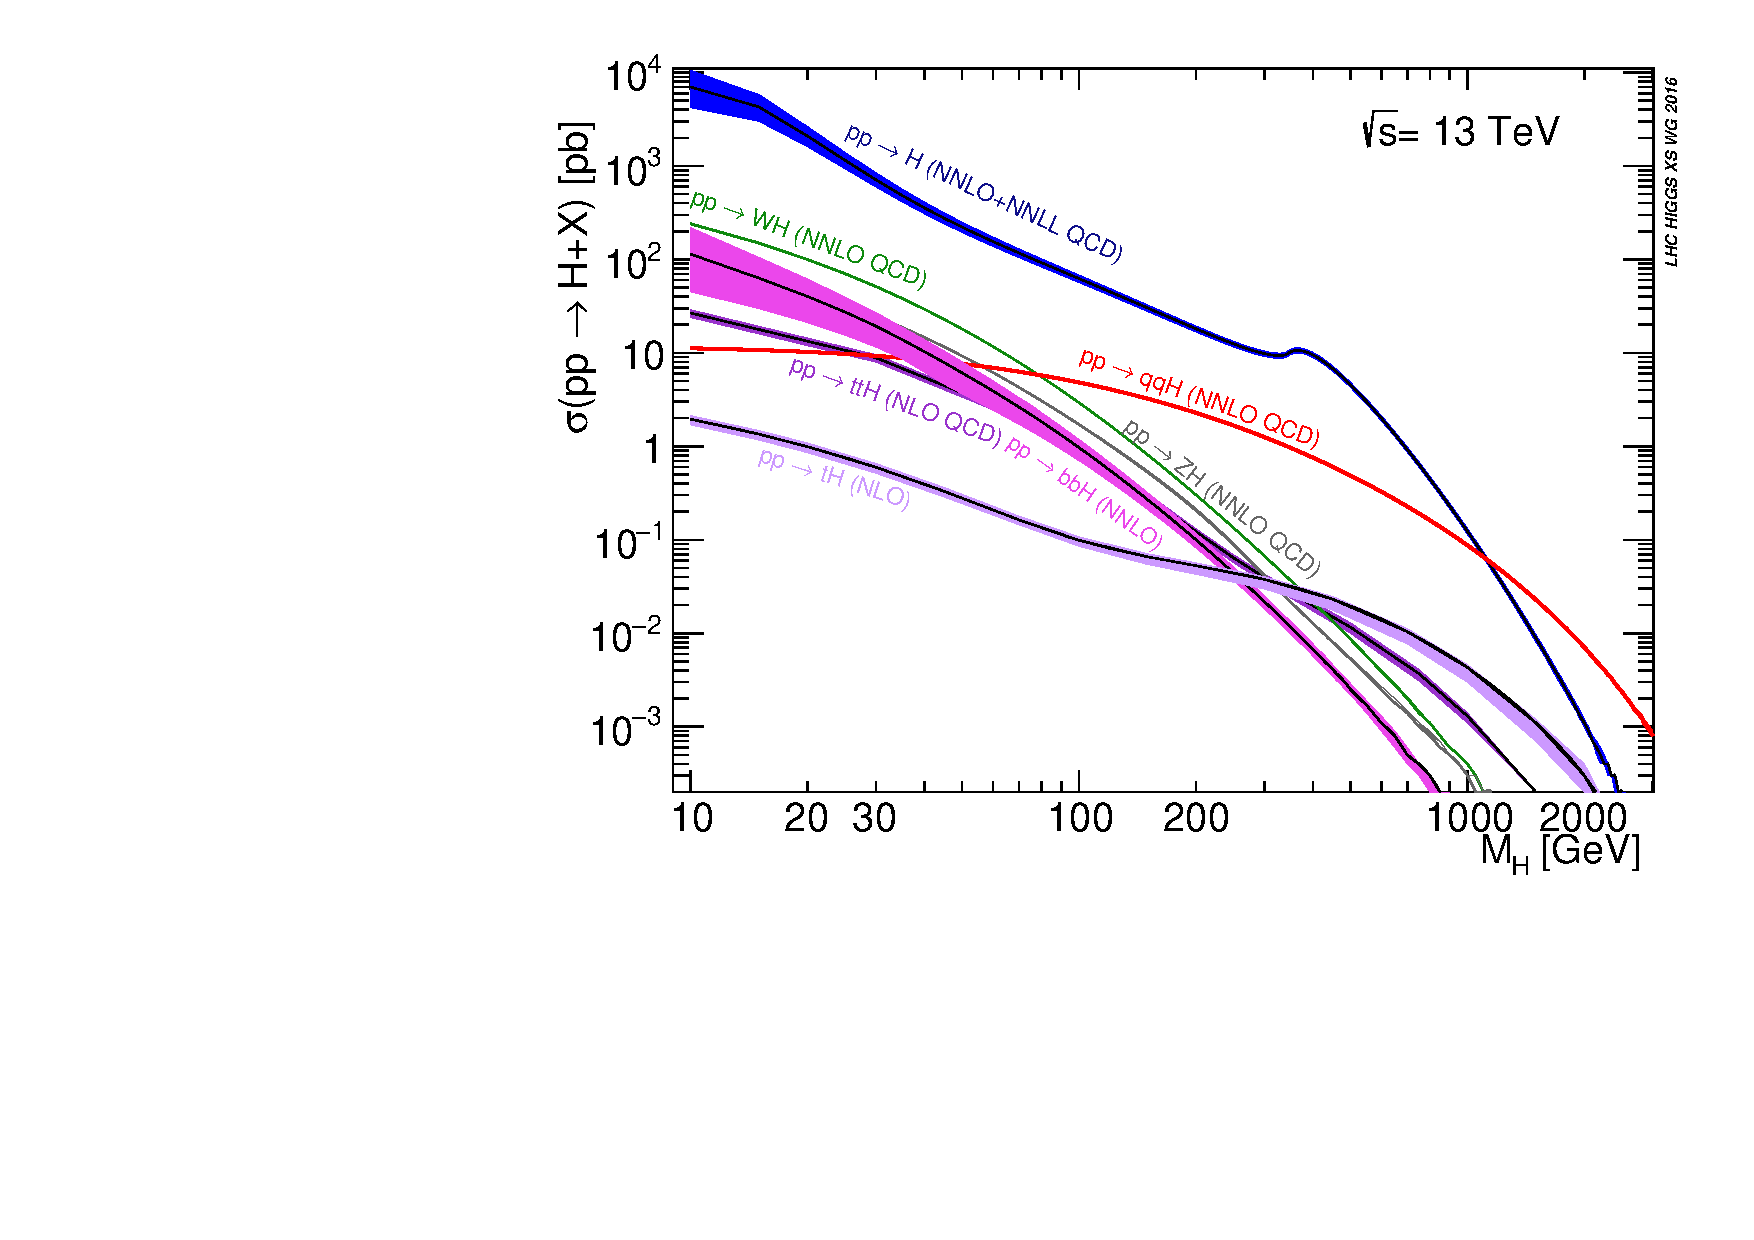
\includegraphics[width=0.45\textwidth]{figures/plotAll_13tev_BSM_sqrt}}
{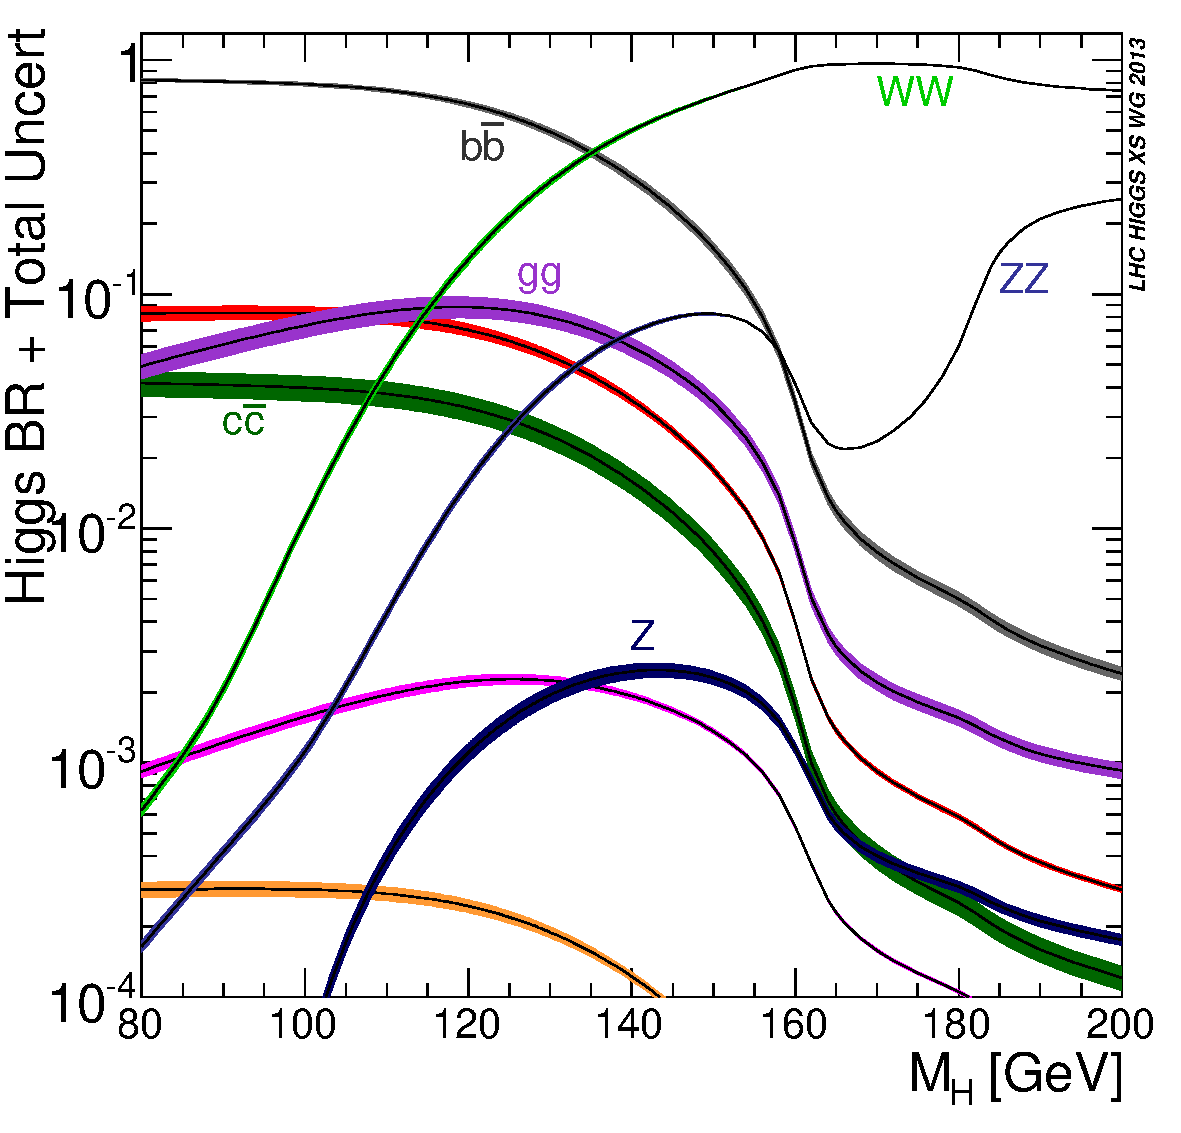
\includegraphics[width=0.4\textwidth]{figures/Higgs_BR_LM}}
\caption{ (Left) The Higgs production cross section, as a function of the Higgs boson mass, for proton-proton colliders at 13 TeV. (Right) The Higgs branching fractions to SM particles, as a function of the Higgs boson mass. }
\label{fig:hig_br_xsec}      
\end{figure}    


Even though the Higgs boson only directly couples to massive particles, processes via loops allow decays such as $H\rightarrow\gamma\gamma$ and production mechanisms such as $gg\rightarrow H$, where $g$ are gluons. 
The latter example is particularly important, since it is the production mechanism with highest cross section at the Large Hadron Collider, a proton-proton collider. 
For other types of colliders, this picture might be different, such as for the Tevatron (proton-antiproton), in which the main production mechanism was through associated production with an electroweak boson. 


\section{Higgs Physics Current Status}

While the Higgs boson, and the electroweak symmetry breaking mechanism applied to the SM itself, was predicted in the 60s, it wasn't until 2012 that it was experimentally verified. 
The CMS and ATLAS experiments, working at the Large Hadron Collider at CERN, detected statistically significant signals compatible with the SM predictions for the Higgs boson, using approximately 5 fb$^{-1}$ of 7 TeV and 8 TeV data \cite{higgs_cms, higgs_atlas}. 

In 2012, it was not possible to say with certainty that this anomaly was, without a doubt, the SM Higgs. 
However, five years later, the data that has been analyzed by the LHC experiments has confirmed the SM predictions for this new particle, with a mass measured as about $125$ GeV, including its spin (scalar) and CP eigenvalue (even) \cite{spin_cms, spin_atlas}. 

The Higgs boson decays to electroweak bosons, $H\rightarrow WW$, $H\rightarrow ZZ$ and $H\rightarrow \gamma\gamma$, have been measured and these branching fractions, assuming SM-like cross section, match the expected values. 
The Higgs decay modes to pairs of fermions have yet to be detected with the statistical significance seen in its bosonic modes. 
However, decays involving the third generation of quarks and leptons, $H\rightarrow b\bar{b}$ and $H\rightarrow \tau\tau$, have seen evidence of such processes when combining searches in different production channels. 
The latest results summary published by CMS and ATLAS can bee seen in Figure \ref{fig:hig_run1_summary} in terms of signal strengths ($\mu$), defined as the ratio of the measured Higgs boson rate to its SM prediction \cite{higgs_pros_cms_atlas}.

\begin{figure}[H]        
\centering                
{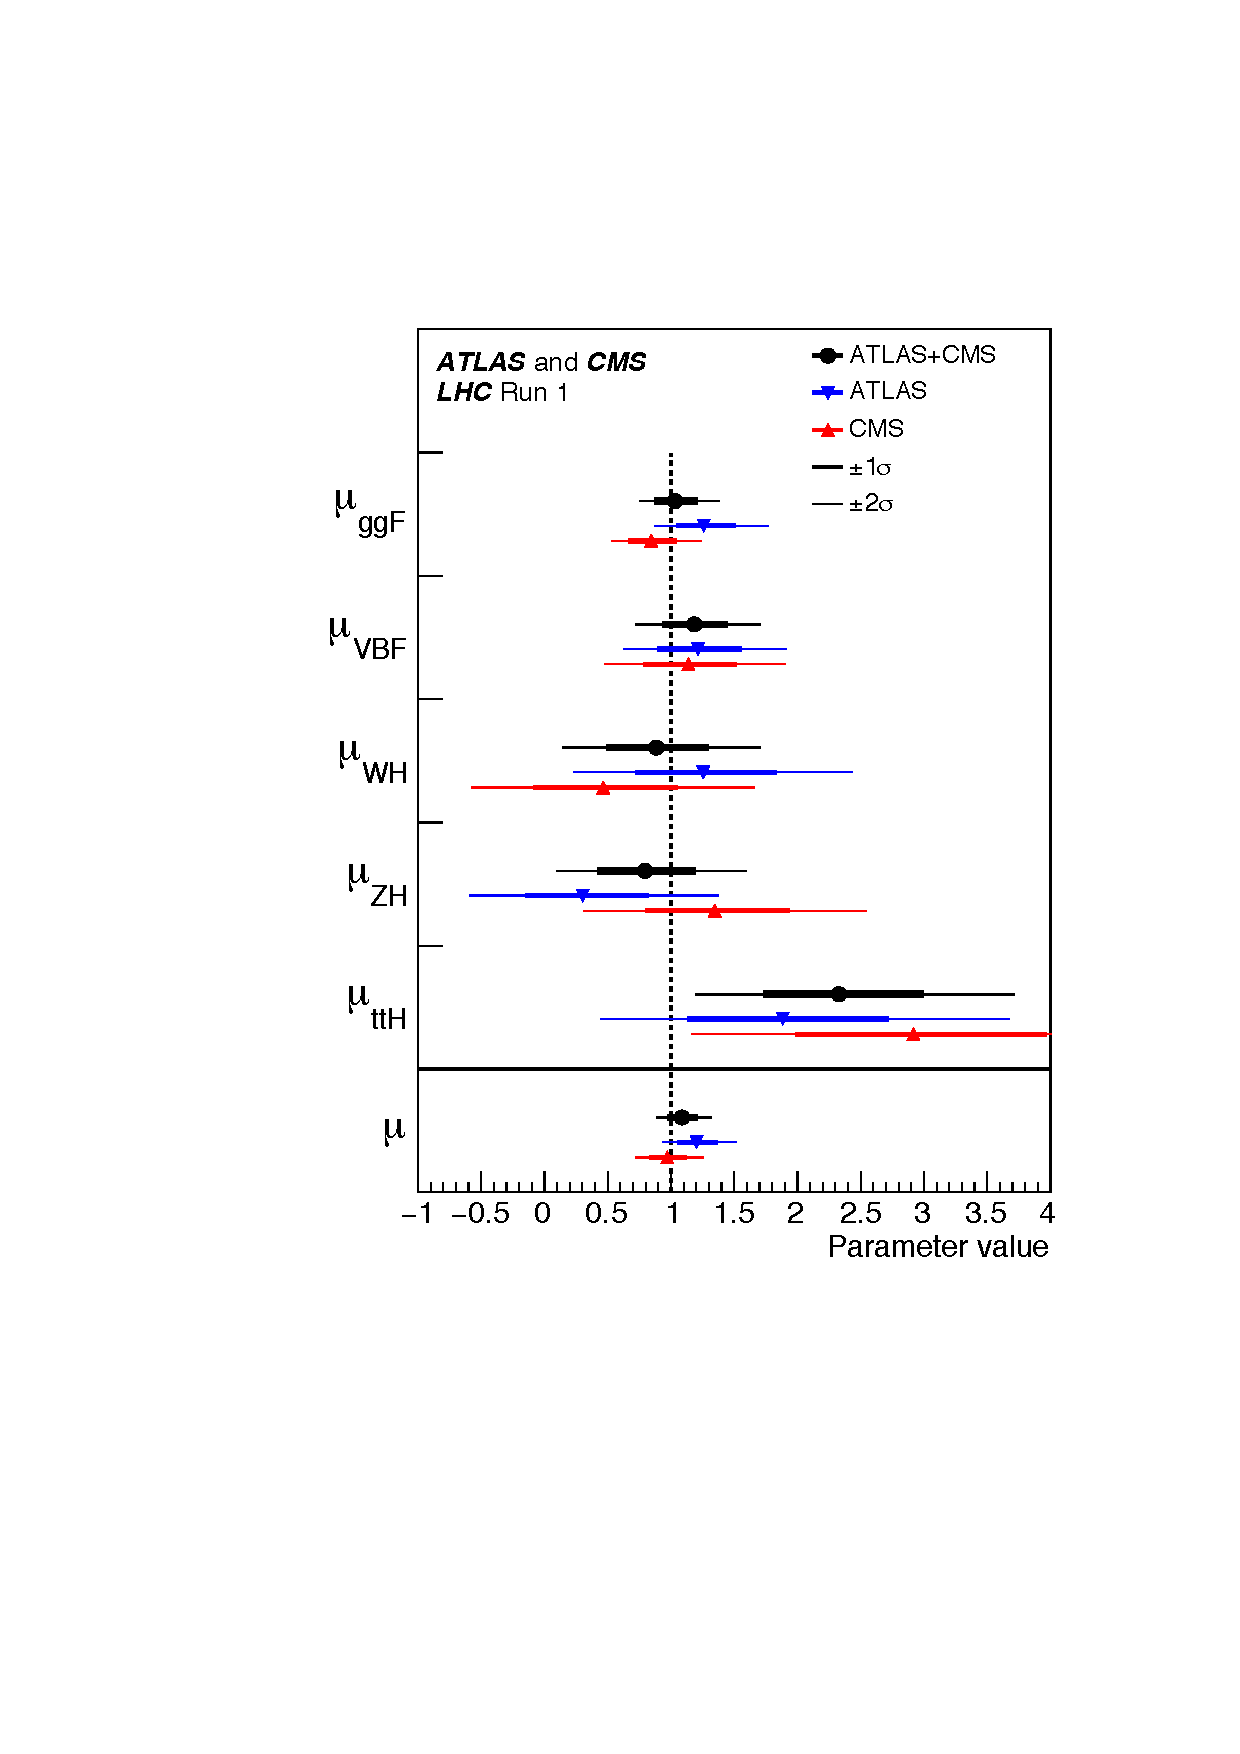
\includegraphics[width=0.45\textwidth]{figures/higgs_prod_run1}}
{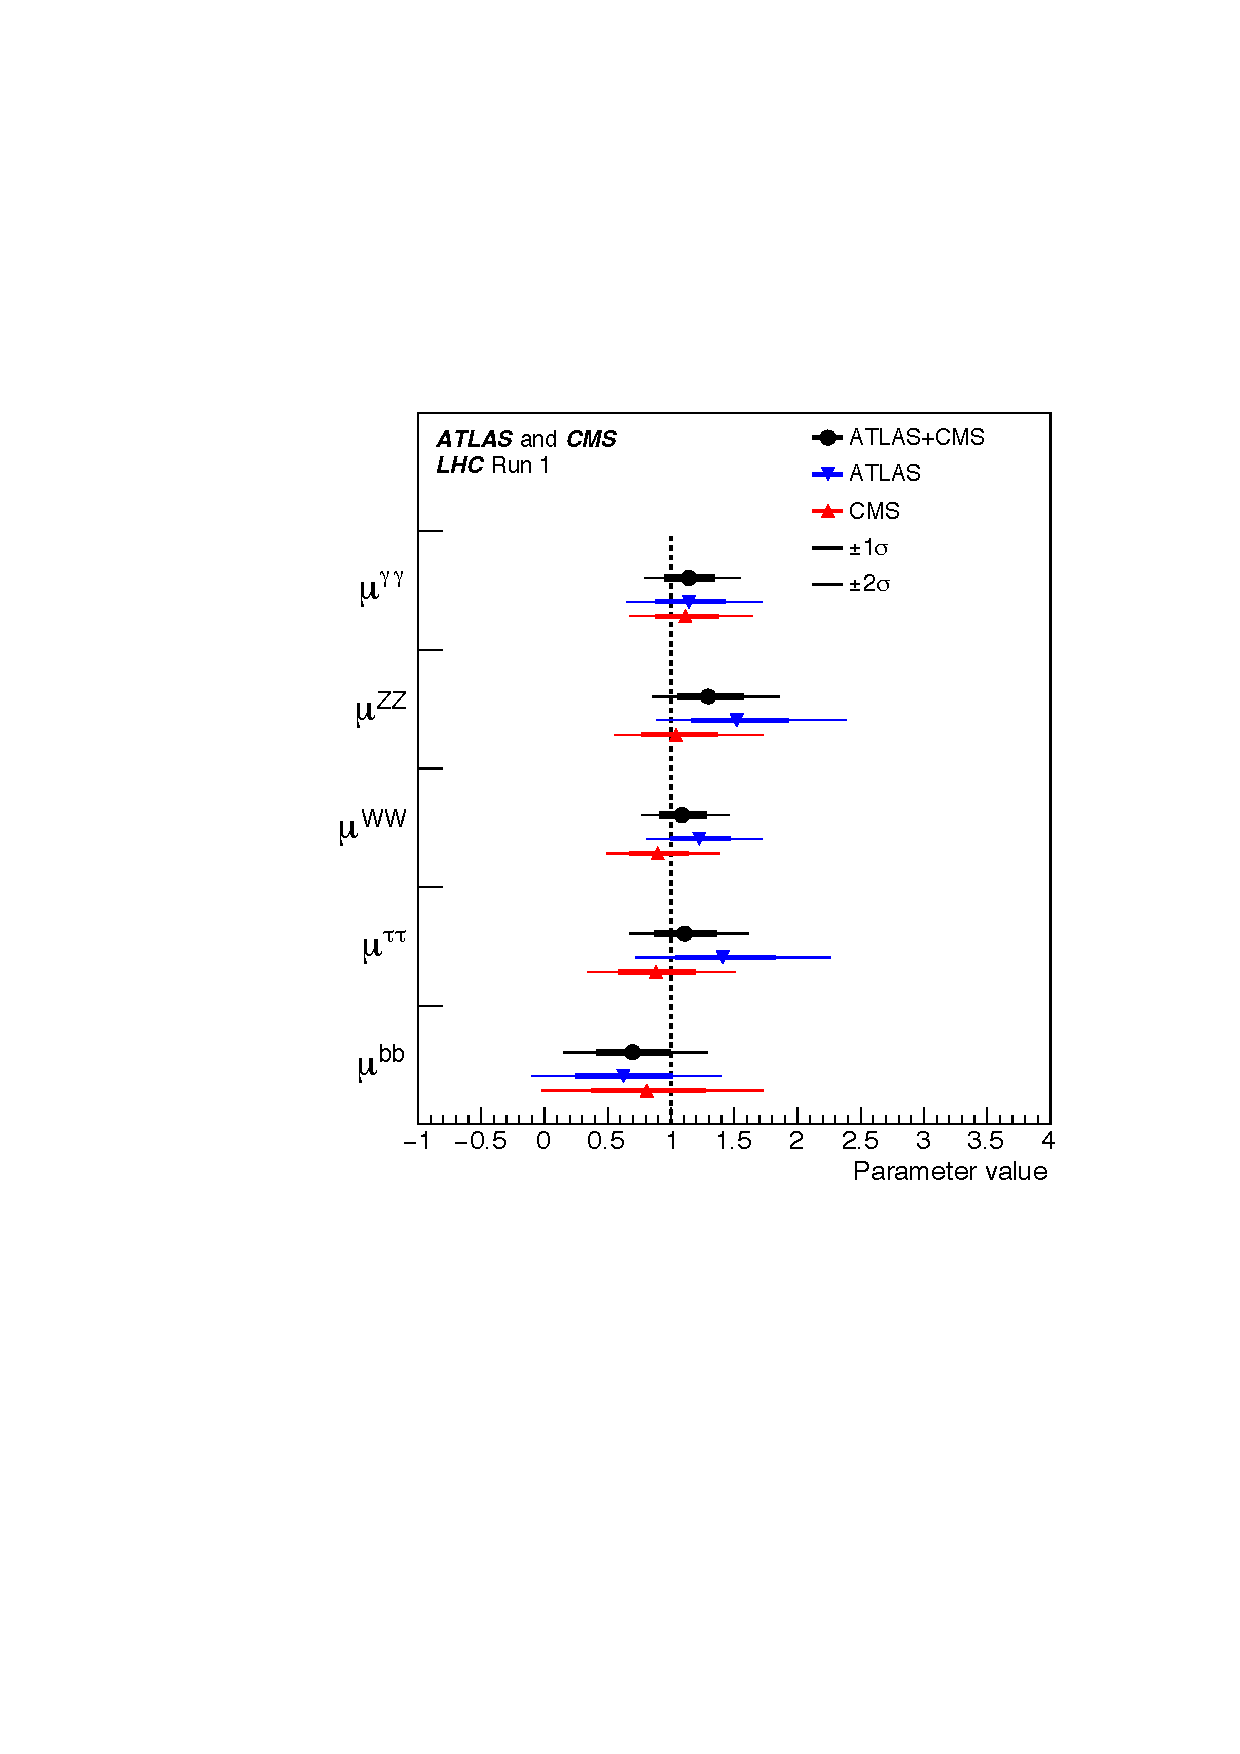
\includegraphics[width=0.45\textwidth]{figures/higgs_decay_run1}}
\caption{ (Left) The signal strength measured for the five main Higgs boson production mechanisms, assuming SM branching fractions. (Right) The signal strength measured for the three bosonic Higgs decays and the two third family fermionic decays, assuming SM production. }
\label{fig:hig_run1_summary}      
\end{figure}    

Other than measuring signal strengths, an important part of studying the Higgs boson is understanding its differential properties. 
Measuring kinematic distributions related to the Higgs candidates, such as the transverse momentum and pseudo-rapidity profiles, can indicate possible corrections and beyond the SM contributions to the production mechanisms. 
For example, new particles appearing in the gluon fusion loop can have different coupling structures that induce kinematic correlations not present in the SM. 
In Figure \ref{fig:hig_diff}, the CMS differential Higgs boson measurements using the $H\rightarrow\gamma\gamma$ channel in terms of the Higgs transverse momentum and rapidity using 8 TeV data \cite{higgs_diff}. 


\begin{figure}[H]        
\centering                
{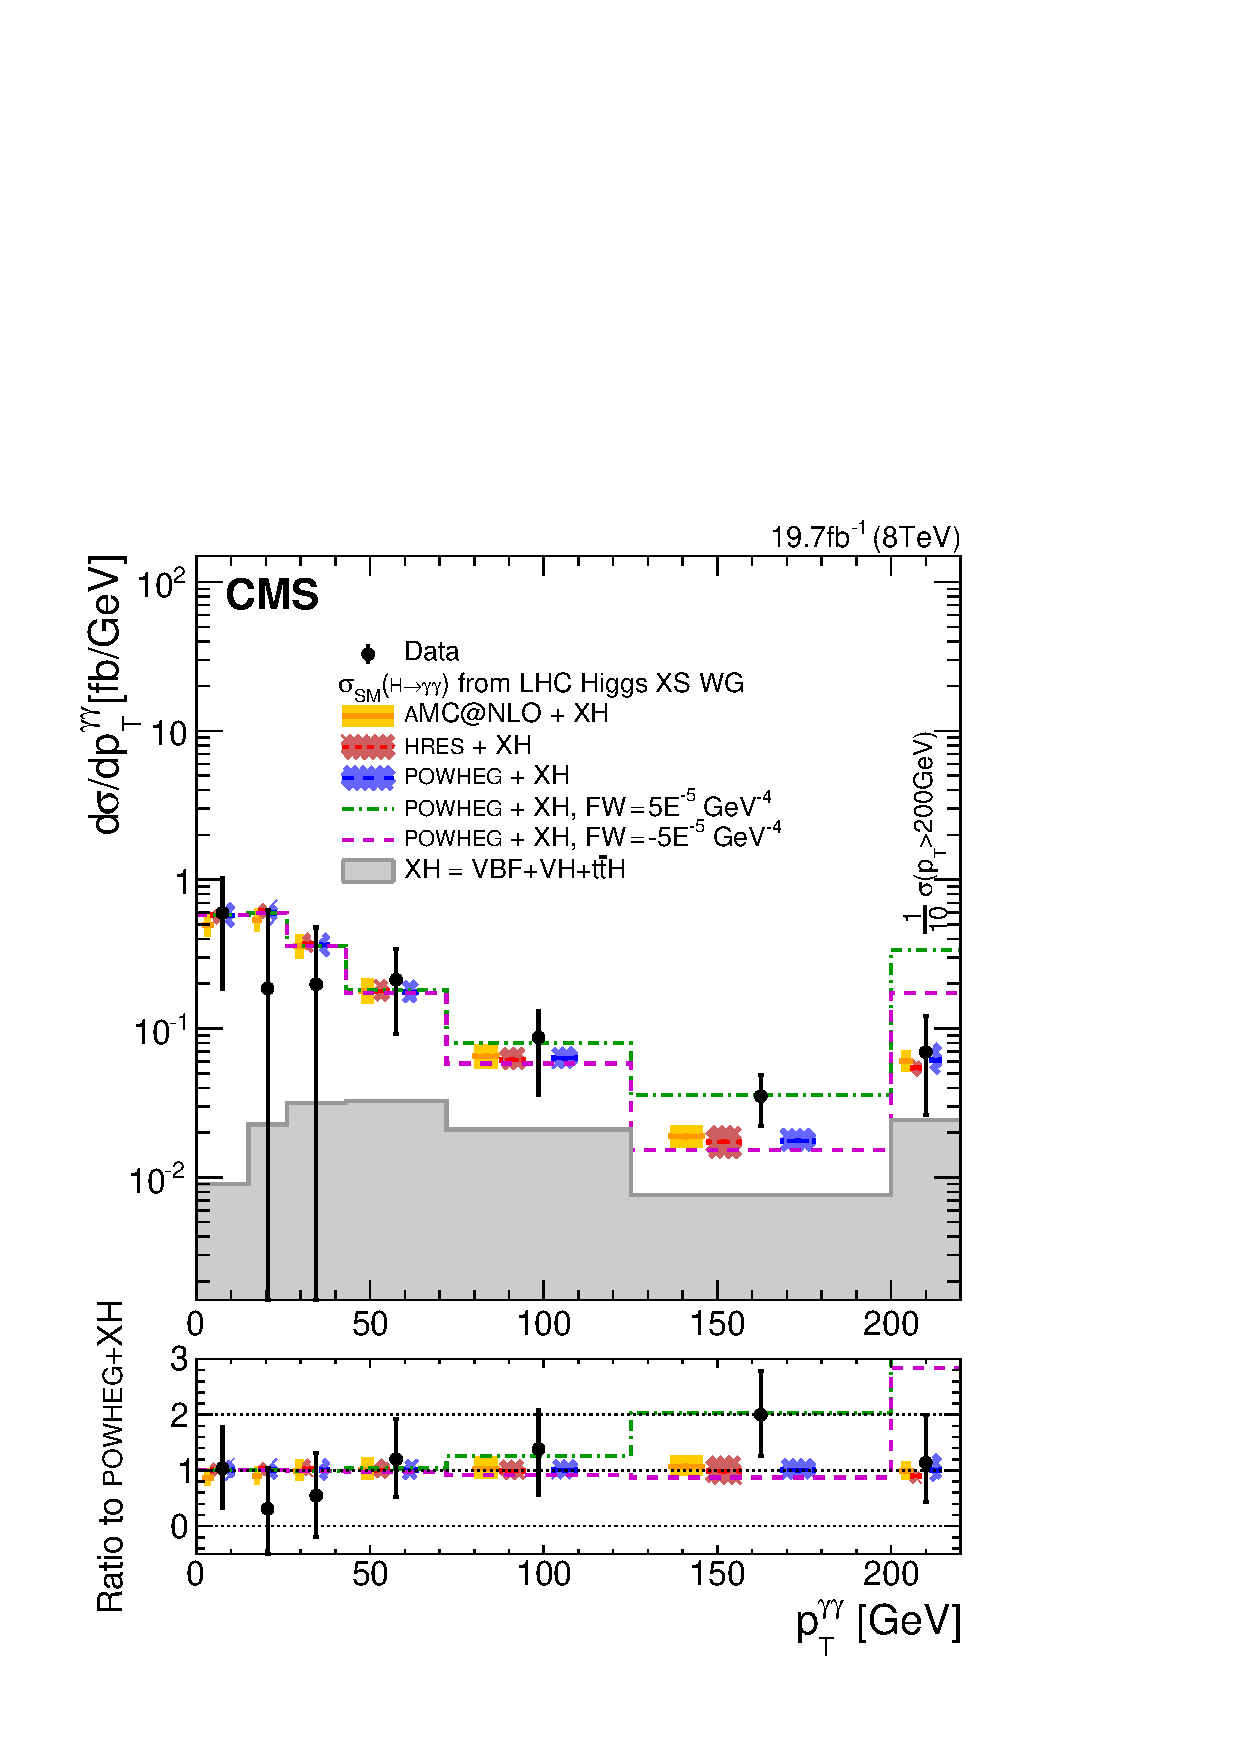
\includegraphics[width=0.45\textwidth]{figures/higgs_diff_pt}}
{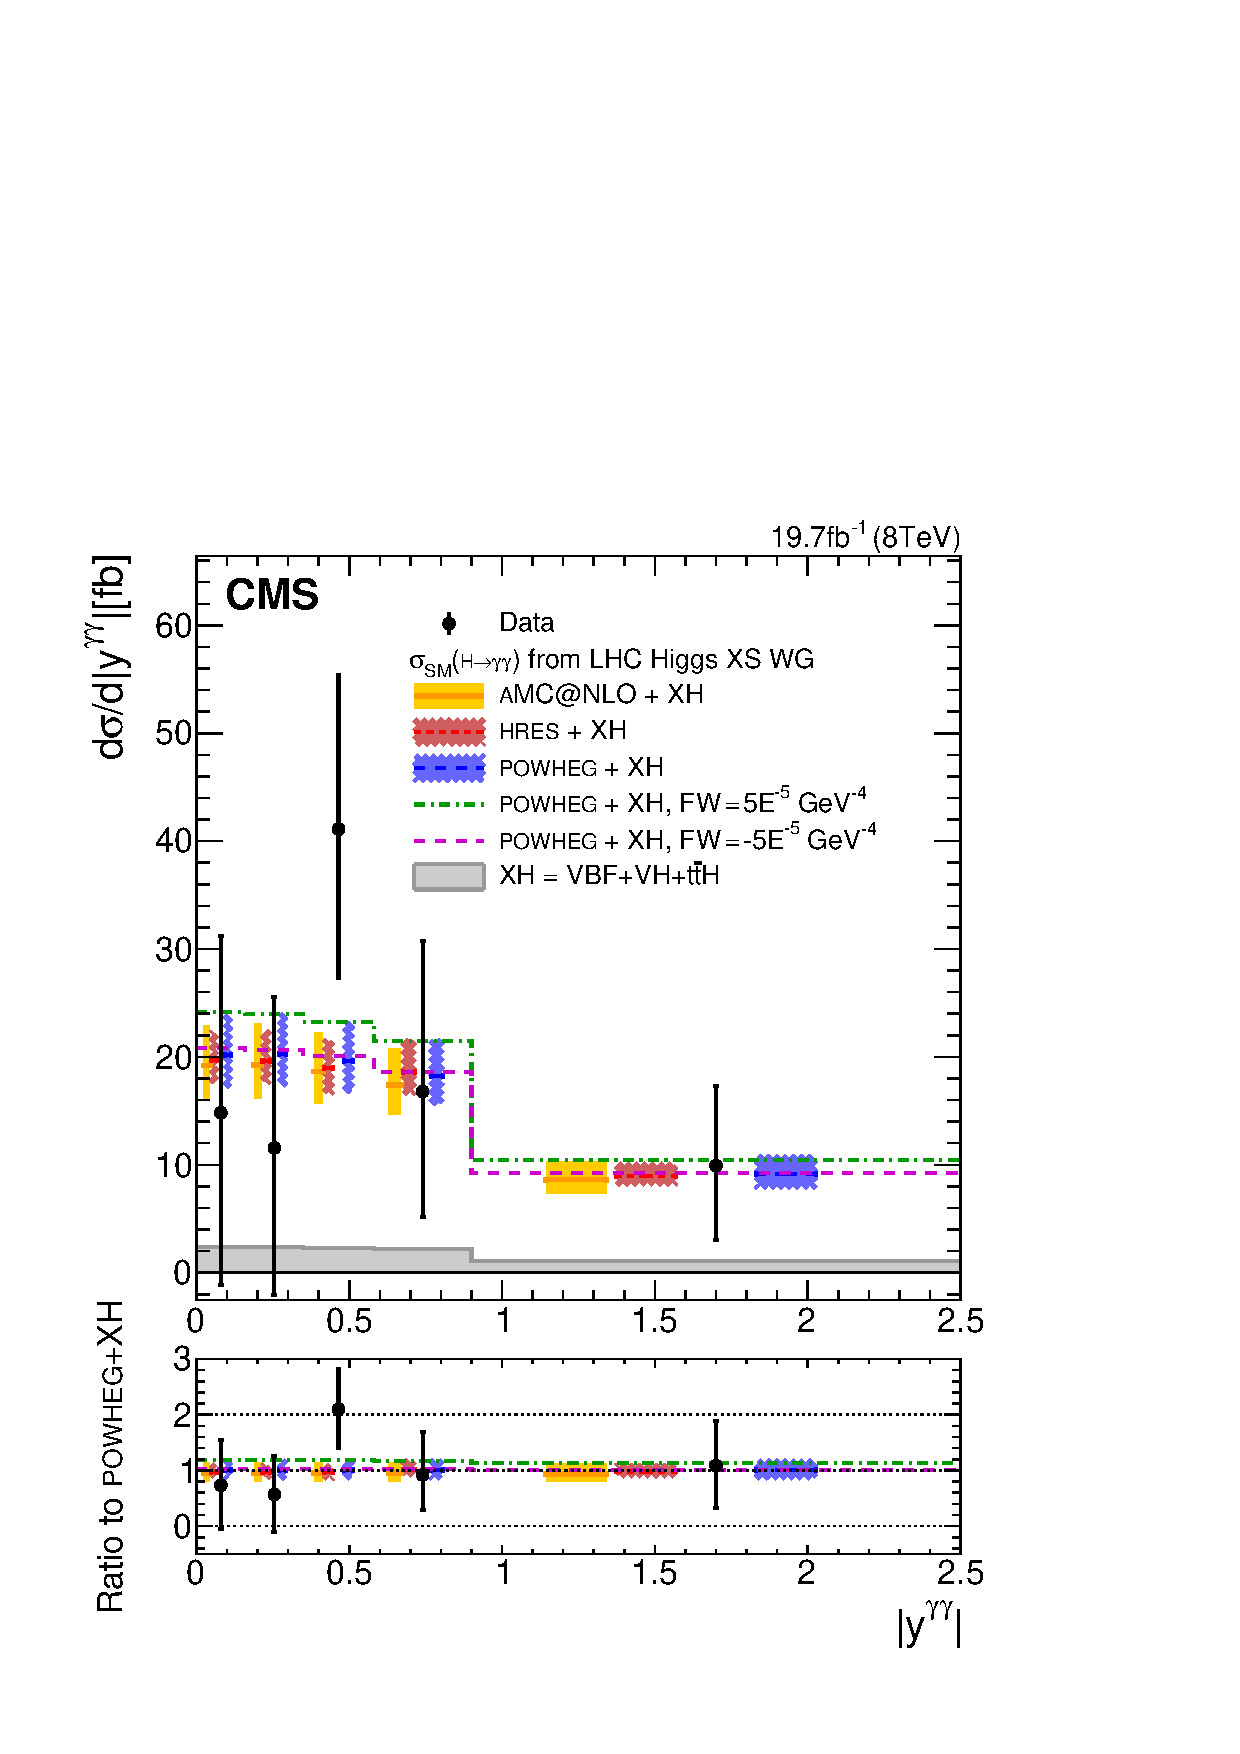
\includegraphics[width=0.45\textwidth]{figures/higgs_diff_rap}}
\caption{ CMS differential Higgs boson measurements using the $H\rightarrow\gamma\gamma$ channel in terms of the Higgs transverse momentum (left) and rapidity (right) using 8 TeV data. The measurements are compared to different Monte Carlo generators. }
\label{fig:hig_diff}      
\end{figure}    



\section{Higgs as a Probe of New Physics}

The experimental confirmation of the Higgs boson marks another success of the SM. 
However, the measured mass of the Higgs boson poses a naturalness conundrum: being a scalar, the Higgs mass is subject to higher order corrections from loops that contain spin 0, 1/2 and 1 particles, which diverge as a function os the energy scale.  
If the SM is valid for all energy scales, these corrections would take the Higgs mass to its highest possible energy scale, the Planck scale ($\approx 10^{19}$ GeV), which is in clear contrast with the Higgs mass value known today. 
In principle, it is possible that the higher order corrections to the Higgs mass cancel out in a way to leave $m_{H} = 125$ GeV, however, such an "accidental" fine tuning is not well motivated within the theory. 
The presence of these two distinct and far apart energy scales in the electroweak theory (Higgs mass and electroweak vacuum versus the Planck scale) is called the Hierarchy problem. 

Several models and extensions to the SM have been proposed to solve the Hierarchy problem. 
Among them, and perhaps the most famous, is Supersymmetry (SUSY) \cite{GGMa,GGMd2,GGMd3,GGMd4,GGMd5,GGMd1,GGMd}. 
SUSY explains the higher order cancelations by postulating a new symmetry of nature that correlates bosons and fermions. 
By symmetrizing the bosonic and fermionic contributions to the Higgs mass corrections, the higher order terms are canceled out naturally (since fermion loops contribute with an overall minus sign relative to boson loops). 

The existence of SUSY implies that, for every elementary fermion in nature, there must exist a boson superpartner with the same mass (same applies to bosons and fermion superpartners). 
However, this has not been observed, which means that, if SUSY exists, it must be a broken symmetry. 
In order to still address the Hierarchy problem, the SUSY breaking scale must be such that the superpartner masses should not exceed $\mathcal{O}(1$ TeV$)$. 
This requirement also has the feature that it unifies the QCD and electroweak coupling constants at $\mathcal{O}(10^{16}$ GeV$)$.

The simplest supersymmetric extension of the SM, known as the Minimal Supersymmetric SM (MSSM), adds the minimal amount of extra fields to the current model to realized SUSY - in the MSSM, each SM fermion/boson will have one boson/fermion superpartner. 
It also introduces changes to the Higgs sector: two Higgs doublets are required in order to perform the electroweak symmetry breaking, and give masses to both up and down type quarks and leptons. 
The existence of this extra doublet now implies that, instead of one Higgs boson mass state, five new bosons exist: two neutral CP-even bosons: $h$, $H$ (one of which is usually identified as the particle discovered in 2012); one neutral CP-odd boson (pseudoscalar): $A$; and two charged charged bosons: $H^{\pm}$. 

The MSSM is one example of model that adds to the Higgs sector of the SM an extra scalar doublet. 
Models with this characteristic are generally referred as Two-Higgs Doublet Models (2HDM) \cite{2hdm}. 
These models are also characterized by new phenomena related to the SM-like Higgs boson, either by exotic production or decay. 
For the first case to happen, at least one of the new resonances in the model, $H$ for example, must be heavier than the SM-like Higgs ($h$), which then allows decays such as $H\rightarrow h+X$, where $X$ can either be a $Z$, an $A$ or even another $h$. 
Alternatively, if $A$, for example, is lighter than $m_{h}/2 \approx 62.5$ GeV, decays such as $h\rightarrow AA$ become possible. 

These specific models serve as illustrations of how a modification to the SM can lead to exotic physics to appear in the Higgs sector. 
More generally, looking for new physics with the Higgs boson is a justifiable ansatz in both phenomenological terms - most extensions to the SM predict specific modifications of the Higgs sector - and in theoretical terms - the Higgs sector is intimately tied to some of the most undesirable features of the SM, such as the Hierarchy problem. 
Another one of these undesirable features is the electroweak vacuum stability problem.

The electroweak vacuum in the SM is defined as the vacuum expectation value given by the Higgs potential minimum: $v \approx 246$ GeV. 
Even though the Higgs potential has one global minimum associated to this vacuum, higher order corrections change the shape of this potential and can turn this global minimum into a local minimum. 
The impact of these corrections are mostly dominated by the Higgs-top quark Yukawa coupling, and so, the stability of the electroweak vacuum depends on the Higgs mass and on the top quark mass, as seen in Figure \ref{fig:hig_stab} \cite{vacuum_stab}. 

Given the current values for the Higgs boson and the top quark masses, our universe currently lies at a meta-stable point. 
These instabilities in the electroweak vacuum can have catastrophic consequences to the fate of the universe, since the vector boson masses, and therefore the strength of the weak interactions, are tied to this value. 
If it is indeed confirmed that we live in such a state, with more precise measurements for the mass parameters, new mechanisms must be in place to safeguard the universe against these features.


 \begin{figure}[h]        
\centering                
{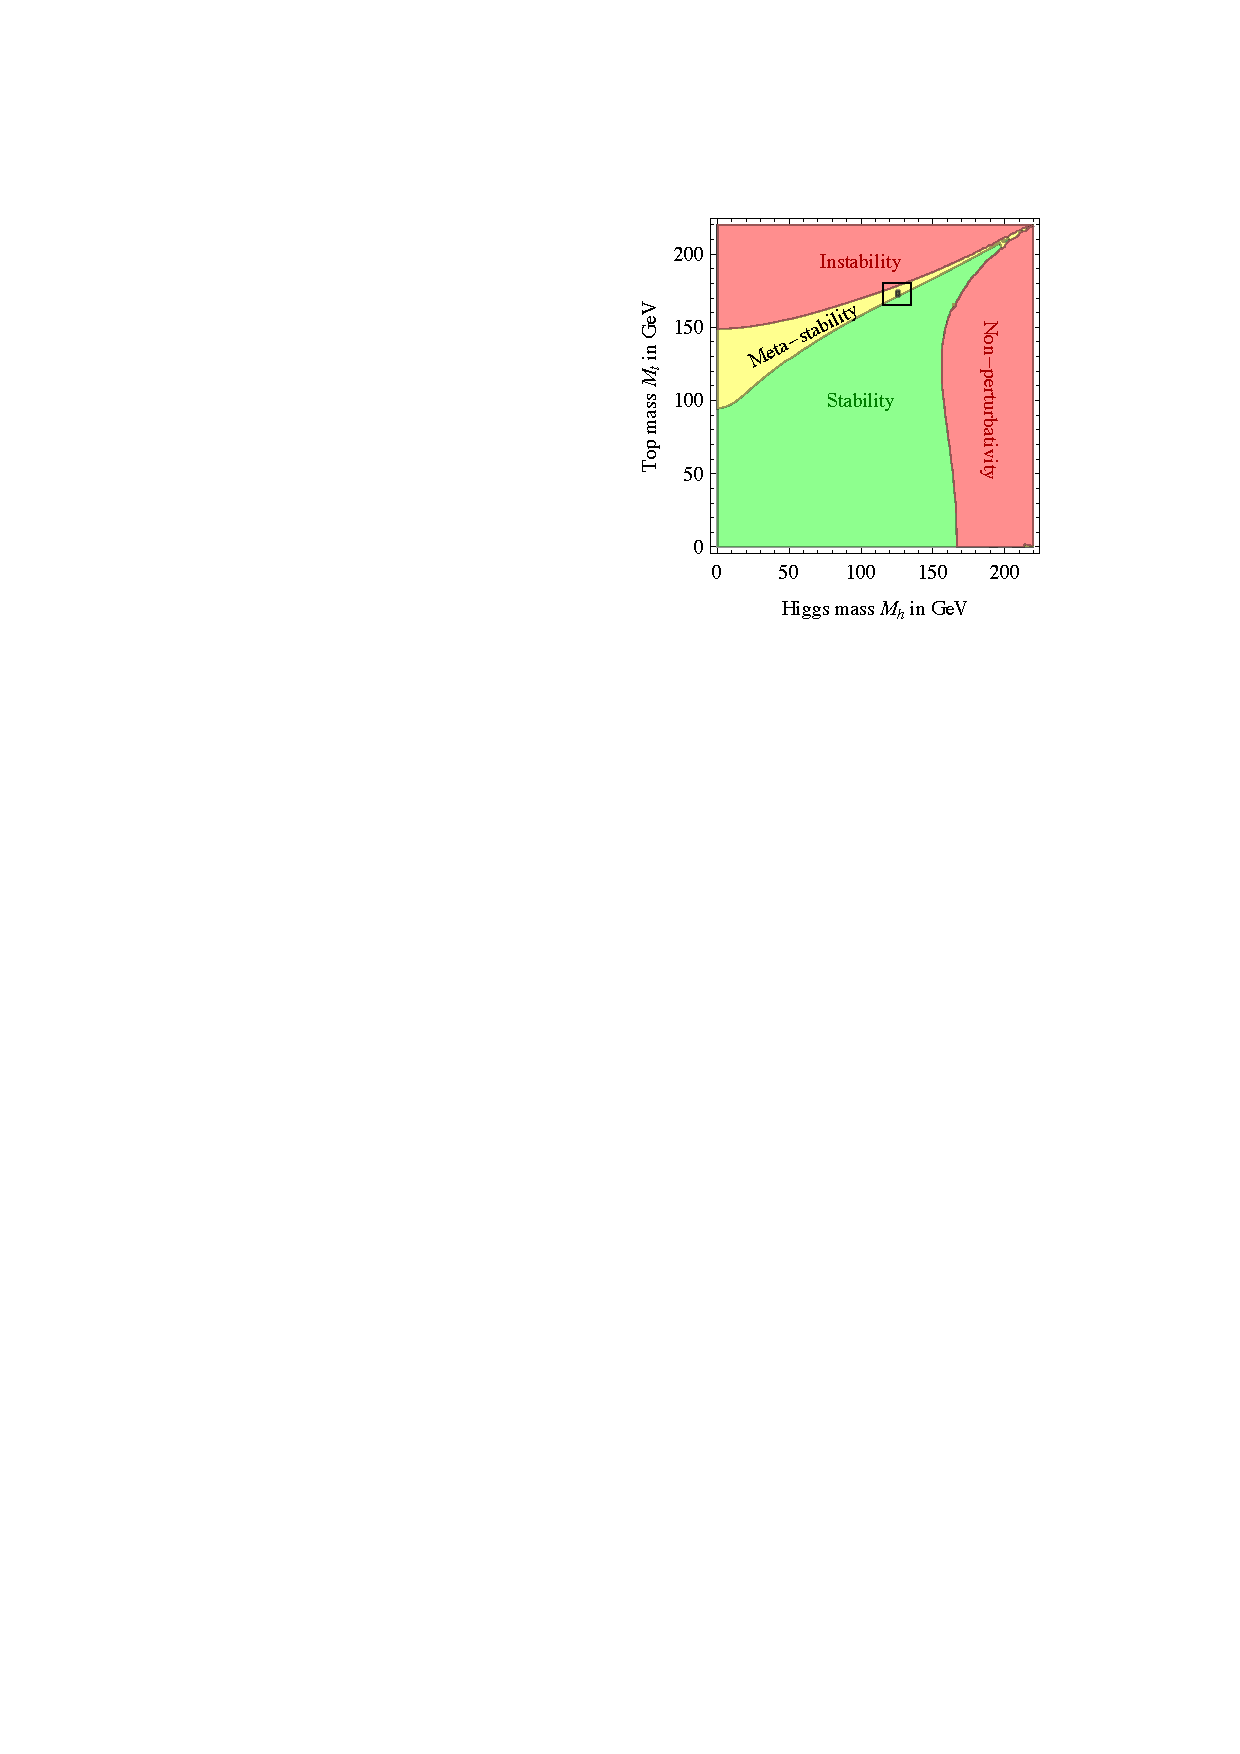
\includegraphics[align=c,width=0.45\textwidth]{figures/higgs_vac_stab}}
{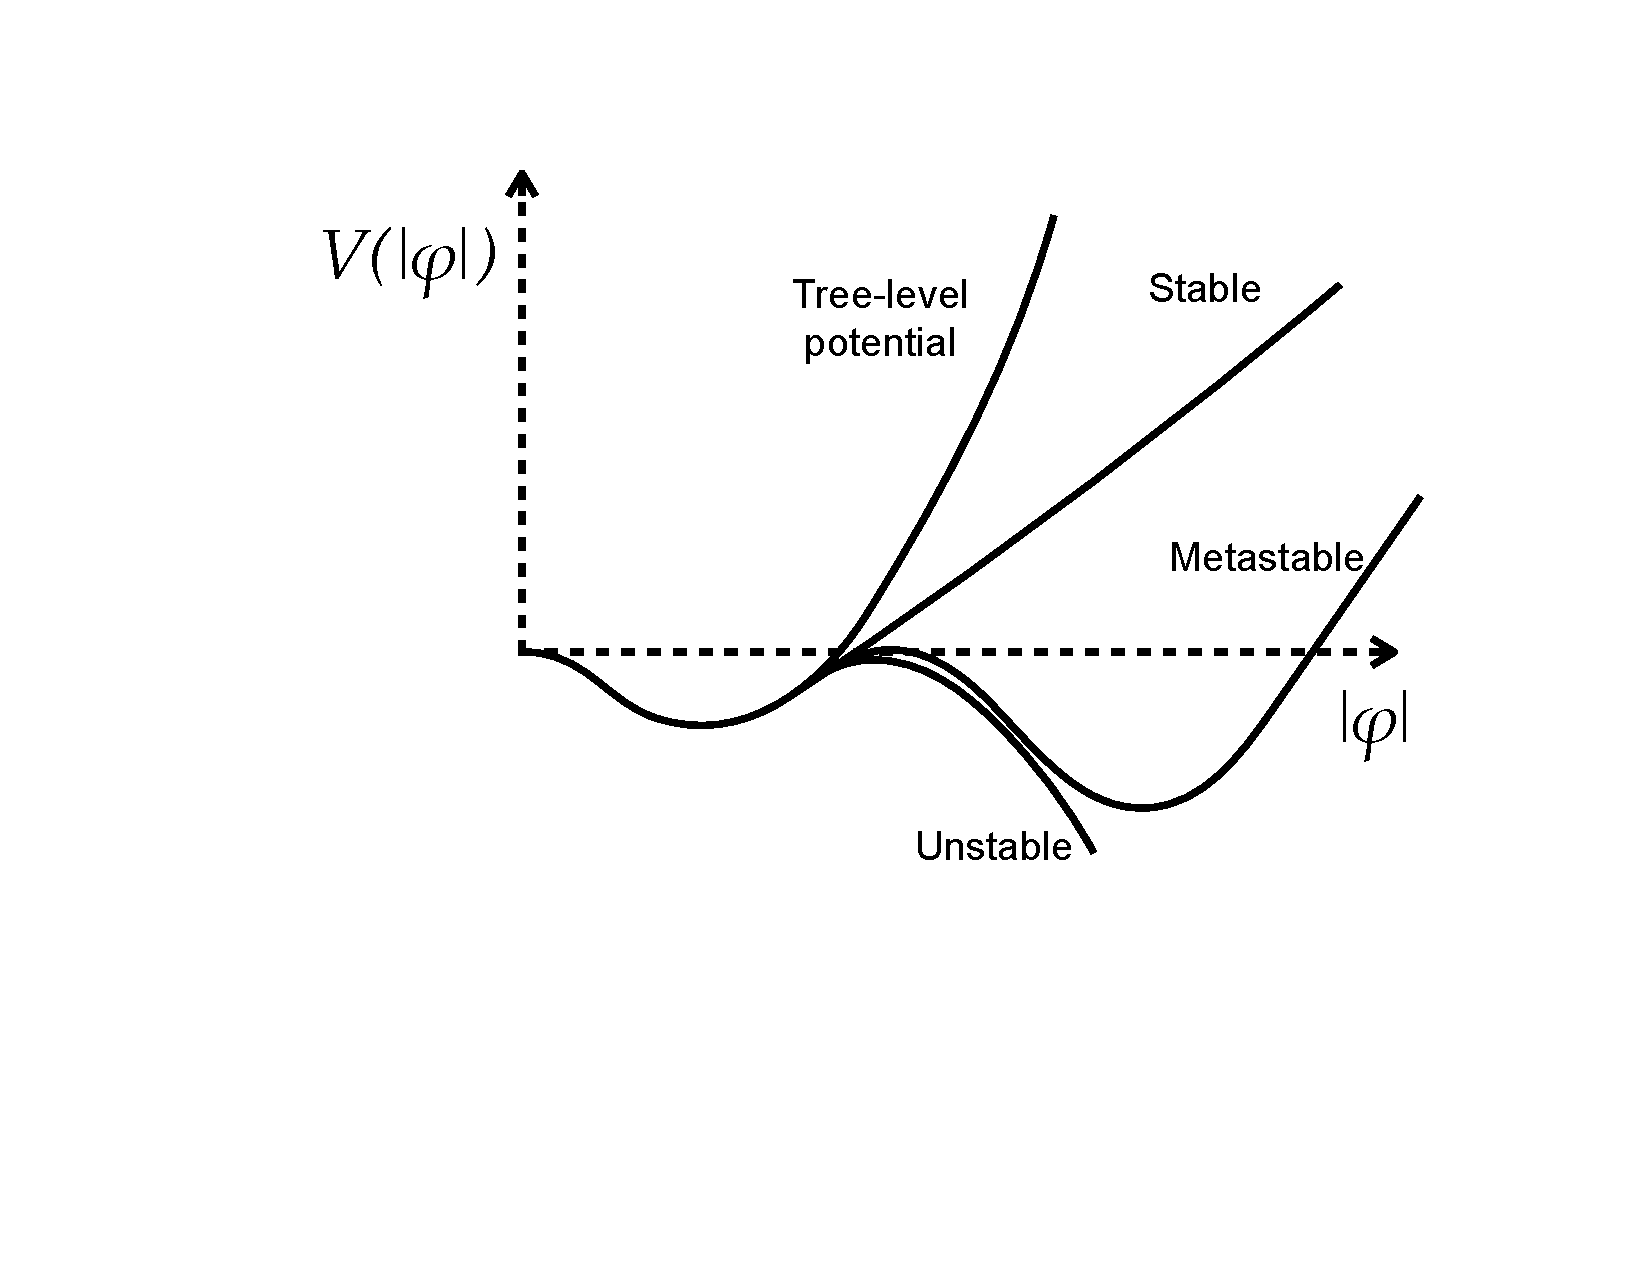
\includegraphics[align=c,width=0.45\textwidth]{figures/higgs_pot_mod}}
\caption{ CMS differential Higgs boson measurements using the $H\rightarrow\gamma\gamma$ channel in terms of the Higgs transverse momentum (left) and rapidity (right) using 8 TeV data. The measurements are compared to different Monte Carlo generators. }
\label{fig:hig_stab}      
\end{figure}    

One important caveat of this stability analysis is the assumption that the tree-level Higgs potential has the quartic shape described in Equation \ref{eq:higgs_pot}. 
However, there are no strong theoretical indications that $V(|\Phi|)$ must have this exact shape. 
Theoretically, the SM $V(|\Phi|)$ is the simplest potential that correctly breaks the electroweak symmetry within theoretical constraints, such as unitarity and renormalizability. 

Experimentally, in order to probe its shape, the $V(|\Phi|)$ potential parameters must be measured directly. 
Through the detection of the Higgs boson and its mass measurement, the parameter $\mu$ in $V(|\Phi|)$ is determined, since $m_{h} = |\mu|$. 
As seen in Equation \ref{eq:higgs_pot_aberto}, the higher order terms of $V(|\Phi|)$ are related to Higgs self-interaction terms. 
It's important to note that, even if the \textit{true} Higgs potential (the one that correctly breaks the electroweak symmetry and brings stability to the SM) is not $V(|\Phi|)$, an expansion of this general potential around the vacuum will generally create higher order terms with respect to $H$. 
Therefore, directly measuring the Higgs self-interaction terms, such as the Higgs triple coupling, is a crucial step towards understanding the SM.




